\PassOptionsToPackage{unicode}{hyperref}
\documentclass[aspectratio=1610, 11pt]{beamer}

\usepackage{amsmath}
\usepackage{amssymb}
\usetheme{tudo}

\title{Datenstrukturen, Algorithmen und Programmierung~2}
\author[A.~Coja-Oghlan]{Amin Coja-Oghlan}
\institute[DAP2]{Lehrstuhl Informatik 2\\Fakult\"at f\"ur Informatik}

\renewcommand{\vec}[1]{\boldsymbol{#1}}
\newcommand\dd{\mathrm d}
\newcommand\eul{\mathrm e}
\newcommand\cA{\mathcal A}
\newcommand\cB{\mathcal B}
\newcommand\cC{\mathcal C}
\newcommand\cD{\mathcal D}
\newcommand\cE{\mathcal E}
\newcommand\cF{\mathcal F}
\newcommand\cG{\mathcal G}
\newcommand\cH{\mathcal H}
\newcommand\cI{\mathcal I}
\newcommand\cJ{\mathcal J}
\newcommand\cK{\mathcal K}
\newcommand\cL{\mathcal L}
\newcommand\cM{\mathcal M}
\newcommand\cN{\mathcal N}
\newcommand\cO{\mathcal O}
\newcommand\cP{\mathcal P}
\newcommand\cQ{\mathcal Q}
\newcommand\cR{\mathcal R}
\newcommand\cS{\mathcal S}
\newcommand\cT{\mathcal T}
\newcommand\cU{\mathcal U}
\newcommand\cV{\mathcal V}
\newcommand\cW{\mathcal W}
\newcommand\cX{\mathcal X}
\newcommand\cY{\mathcal Y}
\newcommand\cZ{\mathcal Z}
\newcommand\fA{\mathfrak A}
\newcommand\fB{\mathfrak B}
\newcommand\fC{\mathfrak C}
\newcommand\fD{\mathfrak D}
\newcommand\fE{\mathfrak E}
\newcommand\fF{\mathfrak F}
\newcommand\fG{\mathfrak G}
\newcommand\fH{\mathfrak H}
\newcommand\fI{\mathfrak I}
\newcommand\fJ{\mathfrak J}
\newcommand\fK{\mathfrak K}
\newcommand\fL{\mathfrak L}
\newcommand\fM{\mathfrak M}
\newcommand\fN{\mathfrak N}
\newcommand\fO{\mathfrak O}
\newcommand\fP{\mathfrak P}
\newcommand\fQ{\mathfrak Q}
\newcommand\fR{\mathfrak R}
\newcommand\fS{\mathfrak S}
\newcommand\fT{\mathfrak T}
\newcommand\fU{\mathfrak U}
\newcommand\fV{\mathfrak V}
\newcommand\fW{\mathfrak W}
\newcommand\fX{\mathfrak X}
\newcommand\fY{\mathfrak Y}
\newcommand\fZ{\mathfrak Z}
\newcommand\fa{\mathfrak a}
\newcommand\fb{\mathfrak b}
\newcommand\fc{\mathfrak c}
\newcommand\fd{\mathfrak d}
\newcommand\fe{\mathfrak e}
\newcommand\ff{\mathfrak f}
\newcommand\fg{\mathfrak g}
\newcommand\fh{\mathfrak h}
%\newcommand\fi{\mathfrak i}
\newcommand\fj{\mathfrak j}
\newcommand\fk{\mathfrak k}
\newcommand\fl{\mathfrak l}
\newcommand\fm{\mathfrak m}
\newcommand\fn{\mathfrak n}
\newcommand\fo{\mathfrak o}
\newcommand\fp{\mathfrak p}
\newcommand\fq{\mathfrak q}
\newcommand\fr{\mathfrak r}
\newcommand\fs{\mathfrak s}
\newcommand\ft{\mathfrak t}
\newcommand\fu{\mathfrak u}
\newcommand\fv{\mathfrak v}
\newcommand\fw{\mathfrak w}
\newcommand\fx{\mathfrak x}
\newcommand\fy{\mathfrak y}
\newcommand\fz{\mathfrak z}
\newcommand\vA{\vec A}
\newcommand\vB{\vec B}
\newcommand\vC{\vec C}
\newcommand\vD{\vec D}
\newcommand\vE{\vec E}
\newcommand\vF{\vec F}
\newcommand\vG{\vec G}
\newcommand\vH{\vec H}
\newcommand\vI{\vec I}
\newcommand\vJ{\vec J}
\newcommand\vK{\vec K}
\newcommand\vL{\vec L}
\newcommand\vM{\vec M}
\newcommand\vN{\vec N}
\newcommand\vO{\vec O}
\newcommand\vP{\vec P}
\newcommand\vQ{\vec Q}
\newcommand\vR{\vec R}
\newcommand\vS{\vec S}
\newcommand\vT{\vec T}
\newcommand\vU{\vec U}
\newcommand\vV{\vec V}
\newcommand\vW{\vec W}
\newcommand\vX{\vec X}
\newcommand\vY{\vec Y}
\newcommand\vZ{\vec Z}
\newcommand\va{\vec a}
\newcommand\vb{\vec b}
\newcommand\vc{\vec c}
\newcommand\vd{\vec d}
\newcommand\ve{\vec e}
\newcommand\vf{\vec f}
\newcommand\vg{\vec g}
\newcommand\vh{\vec h}
\newcommand\vi{\vec i}
\newcommand\vj{\vec j}
\newcommand\vk{\vec k}
\newcommand\vl{\vec l}
\newcommand\vm{\vec m}
\newcommand\vn{\vec n}
\newcommand\vo{\vec o}
\newcommand\vp{\vec p}
\newcommand\vq{\vec q}
\newcommand\vr{\vec r}
\newcommand\vs{\vec s}
\newcommand\vt{\vec t}
\newcommand\vu{\vec u}
\newcommand\vw{\vec w}
\newcommand\vx{\vec x}
\newcommand\vy{\vec y}
\newcommand\vz{\vec z}
\renewcommand\AA{\mathbb A}
\newcommand\NN{\mathbb N}
\newcommand\ZZ{\mathbb Z}
\newcommand\PP{\mathbb P}
\newcommand\QQ{\mathbb Q}
\newcommand\RR{\mathbb R}
\newcommand\RRpos{\mathbb R_{\geq0}}
\renewcommand\SS{\mathbb S}
\newcommand\CC{\mathbb C}
\newcommand{\ord}{\mathrm{ord}}
\newcommand{\id}{\mathrm{id}}
\newcommand{\pr}{\mathrm{P}}
\newcommand{\Vol}{\mathrm{vol}}
\newcommand\norm[1]{\left\|{#1}\right\|} 
\newcommand\sign{\mathrm{sign}}
\newcommand{\eps}{\varepsilon}
\newcommand{\abs}[1]{\left|#1\right|}
\newcommand\bc[1]{\left({#1}\right)} 
\newcommand\cbc[1]{\left\{{#1}\right\}} 
\newcommand\bcfr[2]{\bc{\frac{#1}{#2}}} 
\newcommand{\bck}[1]{\left\langle{#1}\right\rangle} 
\newcommand\brk[1]{\left\lbrack{#1}\right\rbrack} 
\newcommand\scal[2]{\bck{{#1},{#2}}} 
\newcommand{\vecone}{\mathbb{1}}
\newcommand{\tensor}{\otimes}
\newcommand{\diag}{\mathrm{diag}}
\newcommand{\ggt}{\mathrm{ggT}}
\newcommand{\kgv}{\mathrm{kgV}}
\newcommand{\trans}{\top}
\newcommand{\Karonski}{Karo\'nski}
\newcommand{\Erdos}{Erd\H{o}s}
\newcommand{\Renyi}{R\'enyi}
\newcommand{\Lovasz}{Lov\'asz}
\newcommand{\Juhasz}{Juh\'asz}
\newcommand{\Bollobas}{Bollob\'as}
\newcommand{\Furedi}{F\"uredi}
\newcommand{\Komlos}{Koml\'os}
\newcommand{\Luczak}{\L uczak}
\newcommand{\Kucera}{Ku\v{c}era}
\newcommand{\Szemeredi}{Szemer\'edi}

\begin{document}

\maketitle

\begin{frame}{Heapsort}
	\begin{exampleblock}{Sortieren nochmal}
		\begin{itemize}
			\item mit Quicksort haben wir einen (in Erwartung) schnellen randomisierten Sortieralgorithmus kennengelernt
			\item mit Heapsort lernen wir einen effizienten \emph{deterministischen} Sortieralgorithmus kennen
			\item Hilfsmittel ist eine (ansatzweise) raffinierte Datenstruktur
		\end{itemize}
	\end{exampleblock}
\end{frame}

\begin{frame}{Heapsort}
	\begin{exampleblock}{Heaps}
		\begin{itemize}
			\item ein Heap ist eine Datenstruktur in Form eines gewurzelten Baums
%			\item dieser Baum entsteht aus einem vollst\"andigen Bin\"arbaum, indem einige der Bl\"atter gel\"oscht werden
			\item die Knoten sind von $1$ bis $n$ durchnumeriert
			\item Knoten $1$ ist die Wurzel
			\item die Kinder von Knoten $i$ sind $2i$ und $2i+1$, falls diese Werte $\leq n$ sind
			\item jeder Knoten hat also h\"ochstens zwei Kinder
			\item der Elternknoten von Knoten $i\geq2$ ist der Knoten $\lfloor i/2\rfloor$
		\end{itemize}
	\end{exampleblock}
\end{frame}

\begin{frame}{Heapsort}
	\hfill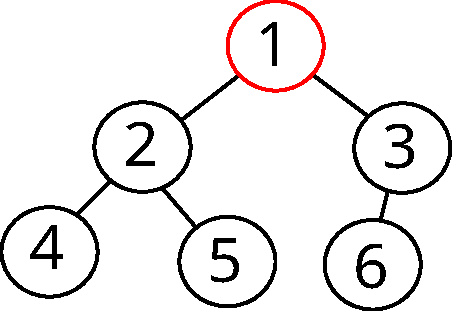
\includegraphics[height=30mm]{./images/heap.pdf}
	\begin{exampleblock}{Beispiel}
		\begin{itemize}
			\item ein Heap mit 6 Knoten
			\item Knoten $1$ ist der Wurzelknoten
		\end{itemize}
	\end{exampleblock}
\end{frame}

\begin{frame}{Heapsort}
	\hfill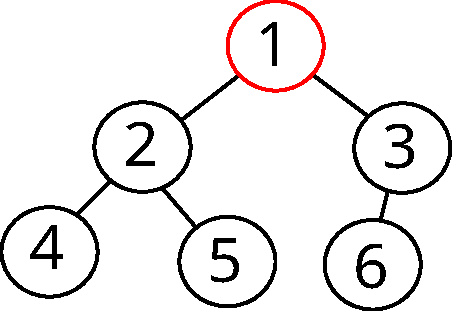
\includegraphics[height=30mm]{./images/heap.pdf}
	\begin{exampleblock}{Repr\"asentation im Speicher}
		\begin{itemize}
			\item ein Heap kann im Speicher einfach in einem \alert{Array} $\vA=(A_1,\ldots,A_n)$ der L\"ange $n$ dargestellt werden
			\item die Indizierung der Eltern/Kinder wird mit den Speicherstellen des Arrays identifiziert
		\end{itemize}
	\end{exampleblock}
\end{frame}

\begin{frame}{Heapsort}
	\begin{exampleblock}{Max-Heaps (und Min-Heaps)}
		\begin{itemize}
			\item in den Knoten des Heaps speichern wir \emph{vergleichbare Werte}
			\item ein \alert{Max-Heap} hat die Eigenschaft, da\ss\ der Wert eines Kindknotens niemals gr\"o\ss er ist als der Wert des Elternknotens
			\item ein \alert{Min-Heap} hat die Eigenschaft, da\ss\ der Wert eines Kindknotens niemals kleiner ist als der Wert des Elternknotens
			\item \emph{wir befassen uns im folgenden nur mit Max-Heaps}
		\end{itemize}
	\end{exampleblock}
\end{frame}

\begin{frame}{Heapsort}
	\begin{exampleblock}{Erzeugen eines Max-Heaps}
		\begin{itemize}
			\item \emph{Aufgabe:} ein Array $\vA=(A_1,\ldots,A_n)$ soll in einen Max-Heap \"uberf\"uhrt werden
			\item {\tt BuildMaxHeap}$(\vA)$ l\"ost dieses Problem f\"ur uns
			\item Hilfsfunktion {\tt MaxHeapify}$(\vA,i)$: die Nachkommen von Knoten $i$ sind bereits Max-Heaps, aber m\"oglicherweise ist der Wert $A_i$ kleiner als der Wert eines Kindes
		\end{itemize}
	\end{exampleblock}
\end{frame}

\begin{frame}{Heapsort}
	\begin{exampleblock}{{\tt MaxHeapify}$(\vA,i)$}
		\begin{enumerate}
			\item Falls $A_i$ nicht kleiner ist als seine Kinder (oder kein Kind hat), halte.
			\item Sonst bestimme das gr\"o\ss ere Kind $A_j$
			\item Vertausche die Werte $A_i$ und $A_j$
			\item {\tt MaxHeapify}$(\vA,j)$
		\end{enumerate}
	\end{exampleblock}
\end{frame}

\begin{frame}{Heapsort}
	\begin{block}{Definition}
		Die \alert{H\"ohe} eines Knotens $i$ ist der maximale direkte Abstand von einem Blatt.
	\end{block}
	\begin{block}{Lemma}
		Die H\"ohe der Wurzel ist $O(\log n)$.		
	\end{block}
\end{frame}

\begin{frame}{Heapsort}
	\begin{block}{Proposition}
		Wenn der Knoten $i$ H\"ohe $h$ hat, ben\"otigt {\tt MaxHeapify}$(\vA,i)$ Laufzeit $O(h)$.
	\end{block}
	\begin{block}{Korollar}
		{\tt MaxHeapify} hat Laufzeit $O(\log n)$.
	\end{block}
\end{frame}

\begin{frame}{Heapsort}
	\begin{exampleblock}{Aufbau eines max-heaps aus einem Array}
		\begin{itemize}
			\item aus einem beliebigen gegebenen Array $\vA$ m\"ochten wir einen max-heap machen
			\item dazu arbeiten wir ``von hinten nach vor''
			\item die letzte H\"alfte der Eintr\"age werden jedenfalls Bl\"atter
			\item auf die anderen Eintr\"age wenden wir {\tt MaxHeapify} an
		\end{itemize}
	\end{exampleblock}
\end{frame}

\begin{frame}{Heapsort}
	\begin{exampleblock}{{\tt BuildMaxHeap}$(\vA)$}
		\begin{enumerate}
			\item F\"ur $i=\lfloor n/2\rfloor,\ldots,1$
			\item $\quad${\tt MaxHeapify}$(\vA,i)$
		\end{enumerate}
	\end{exampleblock}
	\begin{block}{Proposition}
		{\tt BuildMaxHeap} hat Laufzeit $O(n)$
	\end{block}
\end{frame}

\begin{frame}{Heapsort}
	\begin{exampleblock}{{\tt Heapsort}$(\vA)$}
		\begin{enumerate}
			\item {\tt BuildMaxHeap}$(\vA)$
			\item F\"ur $i=n,n-1,\ldots,2$
			\item $\quad$vertausche $A_1$ und $A_i$
			\item $\quad${\tt MaxHeapify}$((A_1,\ldots,A_{i-1}),1)$
		\end{enumerate}
	\end{exampleblock}
	\begin{block}{Satz}
		{\tt Heapsort} sortiert ein gegebenes Array in Zeit $O(n\log n)$
	\end{block}
\end{frame}

\begin{frame}{Heapsort}
	\begin{exampleblock}{Priority queues}
		\begin{itemize}
			\item max-heaps haben weitere Anwendungen
			\item wir versehen die Datenstruktur mit weiteren Operationen
			\item {\tt ExtractMax} (findet und) entfernt das maximale Element
			\item {\tt IncreaseKey} erh\"oht den Wert eines Elements
			\item {\tt Insert} f\"ugt ein neues Element mit einem gegebenen Wert ein
		\end{itemize}
	\end{exampleblock}
\end{frame}

\begin{frame}{Heapsort}
	\begin{exampleblock}{\tt ExtractMax$(\vA)$}
		\begin{enumerate}
			\item falls $n=0$, abbrechen; falls $n=1$, gib $A_1,\emptyset$ aus
			\item vertausche $A_1$ und $A_n$
			\item {\tt MaxHeapify}$((A_1,\ldots,A_{n-1}),1)$
			\item gib $A_n$ und $(A_1,\ldots,A_{n-1})$ aus
		\end{enumerate}
	\end{exampleblock}
\end{frame}

\begin{frame}\frametitle{Heapsort}
	\begin{exampleblock}{\tt IncreaseKey$(\vA,i,\alpha)$}
		\begin{enumerate}
			\item falls $\alpha<A_i$, brich ab
			\item setzte $A_i=\alpha$
			\item solange $i>1$
			\item $\quad$setze $j=\lfloor i/2\rfloor$ \hfill\# $j=$Elternknoten von $A_i$
			\item $\quad$falls $A_j\geq\alpha$, halte
			\item $\quad$falls $A_j<\alpha$, vertausche $A_j$ und $\alpha$
			\item $\quad$setze $i=j$
		\end{enumerate}
	\end{exampleblock}
\end{frame}

\begin{frame}\frametitle{Heapsort}
	\begin{exampleblock}{\tt Insert$(\vA,\alpha)$}
		\begin{enumerate}
			\item f\"uge ein Element $\vA_{n+1}=-\infty$ zu $\vA$ hinzu
			\item wende {\tt IncreaseKey}$((A_1,\ldots,A_{n+1},n+1,\alpha)$ an
		\end{enumerate}
	\end{exampleblock}
\end{frame}

\begin{frame}\frametitle{Heapsort}
	\begin{block}{Proposition}
		Die Operationen {\tt ExtractMax}, {\tt IncreaseKey}, {\tt Insert} haben Laufzeit $O(\log n)$.
	\end{block}
\end{frame}

\begin{frame}\frametitle{Heapsort}
	\begin{exampleblock}{Zusammenfassung}
		\begin{itemize}
			\item {\tt Heapsort} ist ein deterministischer Sortieralgorithmus mit Laufzeit $O(n\log n)$
			\item wesentlicher Baustein ist die max-heap Datenstruktur
			\item diese haben wir zu einer Priority Queue erweitert
		\end{itemize}
	\end{exampleblock}
\end{frame}
\end{document}
